\documentclass{article}

\usepackage{arxiv}

\usepackage[utf8]{inputenc} % allow utf-8 input
\usepackage[T1]{fontenc}    % use 8-bit T1 fonts
\usepackage{hyperref}       % hyperlinks
\usepackage{url}            % simple URL typesetting
\usepackage{booktabs}       % professional-quality tables
\usepackage{amsfonts}       % blackboard math symbols
\usepackage{amsmath}
\usepackage{nicefrac}       % compact symbols for 1/2, etc.
\usepackage{microtype}      % microtypography
\usepackage{graphicx}
\usepackage{float}
\usepackage[numbers]{natbib}
\usepackage{doi}

\renewcommand{\headeright}{}
\renewcommand{\undertitle}{}
\title{SENTIMENT ANALYSIS OF INDONESIAN SPOTIFY REVIEWS USING MACHINE LEARNING AND BILSTM}

\author{%
  \textbf{Uliano Wilyam Purba}\\
  Department of Data Science\\
  Faculty of Science\\
  Sumatera Institute of Technology\\
  Lampung, Indonesia\\
  \texttt{uliano.122450098@student.itera.ac.id}
  \And
  \textbf{Andre Hadiman Rotua Parhusip}\\
  Department of Data Science\\
  Faculty of Science\\
  Sumatera Institute of Technology\\
  Lampung, Indonesia\\
  \texttt{andre.122450108@student.itera.ac.id}
  \And
  \textbf{Sahid Maulana}\\
  Department of Data Science\\
  Faculty of Science\\
  Sumatera Institute of Technology\\
  Lampung, Indonesia\\
  \texttt{sahid.122450109@student.itera.ac.id}
  \And
  \textbf{Luluk Muthoharoh M. Si}\\
  Department of Data Science\\
  Faculty of Science\\
  Sumatera Institute of Technology\\
  Lampung, Indonesia\\
  \texttt{luluk.muthoharoh@sd.itera.ac.id}
  \And
  \textbf{Ardika Satria M. Si}\\
  Department of Data Science\\
  Faculty of Science\\
  Sumatera Institute of Technology\\
  Lampung, Indonesia\\
  \texttt{ardika.satria@sd.itera.ac.id}
  \And
  \textbf{Martin C.T. Manullang Ph.D.}\\
  Department of Informatics Engineering\\
  Faculty of Industrial Technology\\
  Sumatra Institute of Technology\\
  Lampung, Indonesia\\
  \texttt{martin.manullang@if.itera.ac.id}\\
}

\begin{document}
\maketitle

\begin{abstract}
Sentiment analysis of user-generated reviews in morphologically complex, low-resource languages such as Indonesian presents substantial challenges for automated classification systems. This paper presents a systematic benchmarking study comparing three Scikit-learn machine learning classifiers Support Vector Machine (SVM), Multinomial Naive Bayes (MNB), and Decision Tree (DT) --- against a two-layer Bidirectional Long Short-Term Memory (BiLSTM) network implemented in PyTorch, for three-class sentiment classification (Positive, Neutral, Negative) of 100,000 raw Indonesian Spotify reviews (70,155 after deduplication and cleaning) scraped from the Google Play Store. A domain-adapted preprocessing pipeline --- comprising slang normalization, stopword removal, and Sastrawi morphological stemming --- is applied uniformly across both experimental tracks. Classical ML models are evaluated via 5-fold stratified cross-validation on the full 70,155-sample corpus with TF-IDF features and SMOTE class balancing; the BiLSTM (1,096.579 parameters) is trained on a stratified 20,000-sample subset due to CPU-only compute constraints. Among ML classifiers, Decision Tree achieves the highest weighted F1-score of 0.7269, outperforming SVM (0.6958) and MNB (0.4619). The BiLSTM achieves a weighted F1-score of 0.8069 on its held-out test set, surpassing the best ML classifier by +8.0 percentage points on weighted F1. However, the BiLSTM completely fails on the minority Neutral class (F1=0.000) --- a consequence of training without class weighting --- while Decision Tree with SMOTE maintains minimum per-class F1 of 0.707 across all three classes. Results indicate that BiLSTM achieves superior weighted performance for majority-class sentiment discrimination, whereas ML+SMOTE offers more reliable balanced three-class coverage. Both models are deployed as publicly accessible interactive applications on Hugging Face Spaces. This study contributes a transparent, reproducible benchmark for Indonesian app-review sentiment classification under real-world compute-constrained conditions.
\end{abstract}

\keywords{Sentiment Analysis \and Indonesian NLP \and BILSTM \and TF-IDF \and Decision Tree \and Google Play Store Reviews \and PyCaret \and SMOTE \and Class Imbalance \and Hugging Face Deployment}

% ==============================================================================
\section{Introduction}
\label{sec:intro}

Sentiment analysis the task of automatically identifying and categorizing subjective opinions expressed in natural language --- has become one of the most practically consequential subfields of Natural Language Processing (NLP). As mobile application ecosystems continue to expand globally, user-generated reviews on platforms such as the Google Play Store constitute an increasingly rich source of opinion data that developers can leverage to understand user satisfaction, identify recurring pain points, and prioritize product improvements. Automating this process through accurate sentiment classifiers is therefore of direct practical value at scale.

Spotify, one of the world's leading music streaming services, attracts a substantial volume of Indonesian-language reviews from its user base on the Google Play Store. Indonesian presents non-trivial challenges for NLP systems: as an agglutinative language heavily interspersed in informal digital contexts with slang abbreviations, colloquialisms, non-standard orthography, and code-switching with English, it renders tools designed for high-resource languages such as English substantially less effective without targeted, domain-specific preprocessing.

Against this backdrop, a practically important question arises for NLP practitioners: for a real-world Indonesian sentiment classification task of this nature, which paradigm delivers superior performance --- classical machine learning with hand-crafted features, or end-to-end neural sequence modeling? Classical approaches such as Support Vector Machines (SVM), Multinomial Naive Bayes (MNB), and Decision Tree (DT) classifiers, combined with TF-IDF feature extraction, remain widely deployed in production systems due to their interpretability, computational efficiency, and competitive performance on moderate-scale datasets. Deep learning architectures, in particular the Bidirectional Long Short-Term Memory network (BiLSTM), have demonstrated strong sequential text representation capabilities, often achieving superior accuracy when trained on sufficiently large corpora.However, rigorous head-to-head comparisons of these two paradigms specifically on Indonesian mobile application review sentiment classification remain underrepresented in the literature.

This paper presents a systematic benchmarking study comparing three Scikit-learn classifiers --- SVM, MNB, and Decision Tree --- against a two-layer BiLSTM implemented in PyTorch, for three-class sentiment classification (Positive, Neutral, Negative) of 100,000 Indonesian Spotify reviews scraped from the Google Play Store. A key practical dimension of this study is the deliberate and transparent acknowledgment of a training data asymmetry: due to local compute constraints (CPU-only environment), the BiLSTM was trained on a stratified 20,000-sample subset while classical ML models utilized the full 70,155 cleaned samples --- a scenario representative of real-world resource-constrained settings. Both the best-performing ML model and the BiLSTM are deployed as publicly accessible interactive demos on Hugging Face Spaces.

The primary contributions of this work are: (1) a domain-adapted Indonesian text preprocessing pipeline applied consistently across both experimental tracks for fair comparison; (2) a 5-fold cross-validated benchmark of three classical ML classifiers with TF-IDF and SMOTE class balancing on the full 70,155-sample dataset; (3) training and evaluation of a compact BiLSTM model (1,096,579 parameters, well within the $\le10M$ constraint) on a 20,000-sample stratified subset; (4) a transparent comparative analysis including per-class performance breakdown and discussion of minority-class (Neutral) classification failure under both paradigms; and (5) public deployment of both models on Hugging Face Spaces for reproducibility and accessibility.

\begin{itemize}
    \item ML demo: \url{https://huggingface.co/spaces/tubespba-kelompoktuwir/sentimen-spotify-ml}
    \item DL demo: \url{https://huggingface.co/spaces/tubespba-kelompoktuwir/sentimen-spotify-dl}
\end{itemize}

% ==============================================================================
\section{Related Work}
\label{sec:related}

\subsection{Sentiment Analysis: Foundational Work}
The systematic computational treatment of opinion and sentiment in text was formalized by Pang and Lee \cite{pang2008opinion}, whose foundational survey established the key tasks, methodologies, and evaluation frameworks that continue to underpin the field. Their work demonstrated that machine learning approaches particularly Support Vector Machines combined with bag-of-words and TF-IDF features --- could achieve strong performance on document-level sentiment classification, forming the methodological basis for classical NLP pipelines widely adopted thereafter.

\subsection{Classical Machine Learning for Text Classification}
Among classical approaches, the combination of TF-IDF feature extraction with SVM, Multinomial Naive Bayes, and Decision Tree classifiers has proven consistently effective for sentiment and opinion classification tasks. Pratap and Nidhi \cite{pratap2020comparative} demonstrated that SVM with TF-IDF achieves the highest accuracy (93.37\%, F1: 0.88) on Google Play Store app reviews, outperforming Naive Bayes and Logistic Regression variants across n-gram schemes. Similarly, Rustam et al.\ \cite{rustam2021comparative} compared SVM, Logistic Regression, MNB, and 
Random Forest on a large, imbalanced, multi-class Twitter airline dataset, finding  SVM and Logistic Regression superior at 77\% accuracy under BoW and TF-IDF representations. These results highlight that, with appropriate feature engineering, classical models remain competitive baselines for app review sentiment tasks. Our work similarly benchmarks these three classifiers but operates on Indonesian-language reviews, a substantially more challenging linguistic domain.

\subsection{Deep Learning for Sentiment Analysis}
The introduction of Long Short-Term Memory (LSTM) networks by Hochreiter and Schmidhuber \cite{hochreiter1997lstm} addressed the vanishing gradient problem in sequential learning, enabling effective modeling of long-range textual dependencies. The Bidirectional extension (BiLSTM), which processes sequences in both forward and backward directions, further enhanced contextual understanding and became a widely adopted architecture for sentiment classification \cite{xu2019bilstm}. Xu et al. \cite{xu2019bilstm} demonstrated that BiLSTM achieves strong performance on comment sentiment analysis. More recently, Lin and Nuha \cite{lin2023hybrid} proposed a hybrid Bi-LSTM and Temporal Convolutional Network (TCN) architecture for Indonesian sentiment analysis across multiple topic domains, showing that deep sequential models outperform classical baselines when combined with BERT-based text representations, though at substantially higher computational cost.

\subsection{Indonesian NLP and Sentiment Analysis}
Despite Indonesian being the fourth most widely used language on the internet, NLP research for this language has historically been constrained by limited annotated resources \cite{wilie2020indonlu}. Wilie et al.\ \cite{wilie2020indonlu} addressed this gap by introducing IndoNLU, the first comprehensive benchmark suite for Indonesian NLU tasks, including sentiment analysis subtasks (SmSA), and releasing pre-trained IndoBERT models. Within this space, several studies have evaluated deep learning methods for Indonesian sentiment classification. Kuncahyo et al.\ \cite{kuncahyo2020bilstm} applied BiLSTM with paragraph vector representations to document-level Indonesian sentiment analysis, showing improvement over SVM baselines, particularly on ambiguous-polarity texts. Farizki et al. \ \cite{farizki2025bilstm} evaluated BiLSTM and IndoBERT on a limited Indonesian dataset, confirming BiLSTM's strong capacity to capture bidirectional context even without transformer-level pretraining. Most recently, Abiola et al. \ \cite{abiola2024sentiment} benchmarked LSTM, BiLSTM, and GRU on the 2024 Indonesian presidential candidate sentiment dataset, finding BiLSTM superior with 80.70\% accuracy and 86.86\% F1-score --- closely aligned with our own BiLSTM results on Spotify reviews. Morphological stemming for Indonesian, a preprocessing step in both our ML and DL pipelines, relies on the Sastrawi library, which implements the Nazief-Adriani algorithm as extended by the Enhanced Confix Stripping stemmer \cite{adriani2007stemming}.

\subsection{App Review Sentiment Analysis}
Sentiment analysis of mobile application reviews has emerged as a distinct applied domain. Ossai and Wickramasinghe \cite{ossai2024sentiment} conducted sentiment analysis on 33,000 Google Play Store reviews across 15 apps, comparing ANN, LSTM, and SVM with TF-IDF features, finding deep learning models generally superior while noting that classical SVM remains competitive under constrained data conditions. Class imbalance --- a pervasive challenge in real-world review datasets where positive reviews substantially outnumber neutral and negative ones --- is a recurring concern addressed via oversampling techniques such as SMOTE \cite{chawla2002smote}, which we apply in our ML pipeline. To the best of our knowledge, no prior work has conducted a head-to-head benchmark of Scikit-learn ML classifiers against a PyTorch BiLSTM specifically on large-scale Indonesian Spotify review data, with consistent preprocessing and public deployment, making this study a targeted contribution to the Indonesian app-review NLP literature.

% ==============================================================================
\section{Dataset}
\label{sec:dataset}

\subsection{Data Source and Collection}
The dataset used in this study consists of 100,000 Indonesian-language user reviews of the Spotify mobile application scraped from the Google Play Store using the {google-play-scraper} library. Reviews were collected over a period spanning May 2024 to December 2025, capturing a temporally coherent snapshot of user sentiment toward the application. Spotify is the dominant music and podcast streaming platform in Indonesia, competing primarily with YouTube Music and local services such as Joox, making its user review corpus a practically relevant and linguistically rich source for Indonesian NLP research.

\begin{table}[H]
\centering
\caption{Raw Spotify Dataset}
\label{tab:raw_dataset}
\begin{tabular}{cllccc}
\toprule
\textbf{No} & \textbf{Nama User} & \textbf{Ulasan} & \textbf{Rating} & \textbf{Tanggal} & \textbf{Versi App} \\ \midrule
0 & Pengguna Google & suka banget sama ni app & 5 & 2025-12-31 & 9.1.6.1145 \\
1 & Pengguna Google & bgus & 5 & 2025-12-31 & 9.1.6.1145 \\
2 & Pengguna Google & ga bisa denger lagu JKT48 lagi... & 1 & 2025-12-31 & 9.1.6.1145 \\
3 & Pengguna Google & lagunya bagus banget... & 5 & 2025-12-31 & 9.1.6.1145 \\
\vdots & \vdots & \vdots & \vdots & \vdots & \vdots \\
99999 & Pengguna Google & Minimal bisa di pake pas make data... & 2 & 2024-05-23 & 9.40.509 \\ \bottomrule
\end{tabular}
\end{table}

The raw dataset comprises six columns: Nama User (reviewer username), Ulasan (review text in Bahasa Indonesia), Rating (integer star rating, 1–5), Tanggal (review timestamp), Likes (number of upvotes received), and Versi App (installed Spotify version at time of review). For the purposes of this study, only the Ulasan and Rating columns are used as inputs to the classification pipeline.

\subsection{Sentiment Label Construction}
Following standard practice in rating-based sentiment labeling [1, 2], star ratings are mapped to three ordinal sentiment classes: ratings of 1-2 are labeled Negatif (Negative), rating 3 is labeled Netral (Neutral), and ratings of 4-5 are labeled Positif (Positive). This three-class scheme reflects the natural interpretation of app store ratings and is consistent with the sentiment taxonomy adopted in Indonesian NLP benchmarks such as IndoNLU [7].

\subsection{Dataset Statistics and Class Distribution}
\begin{figure}[H]
\centering
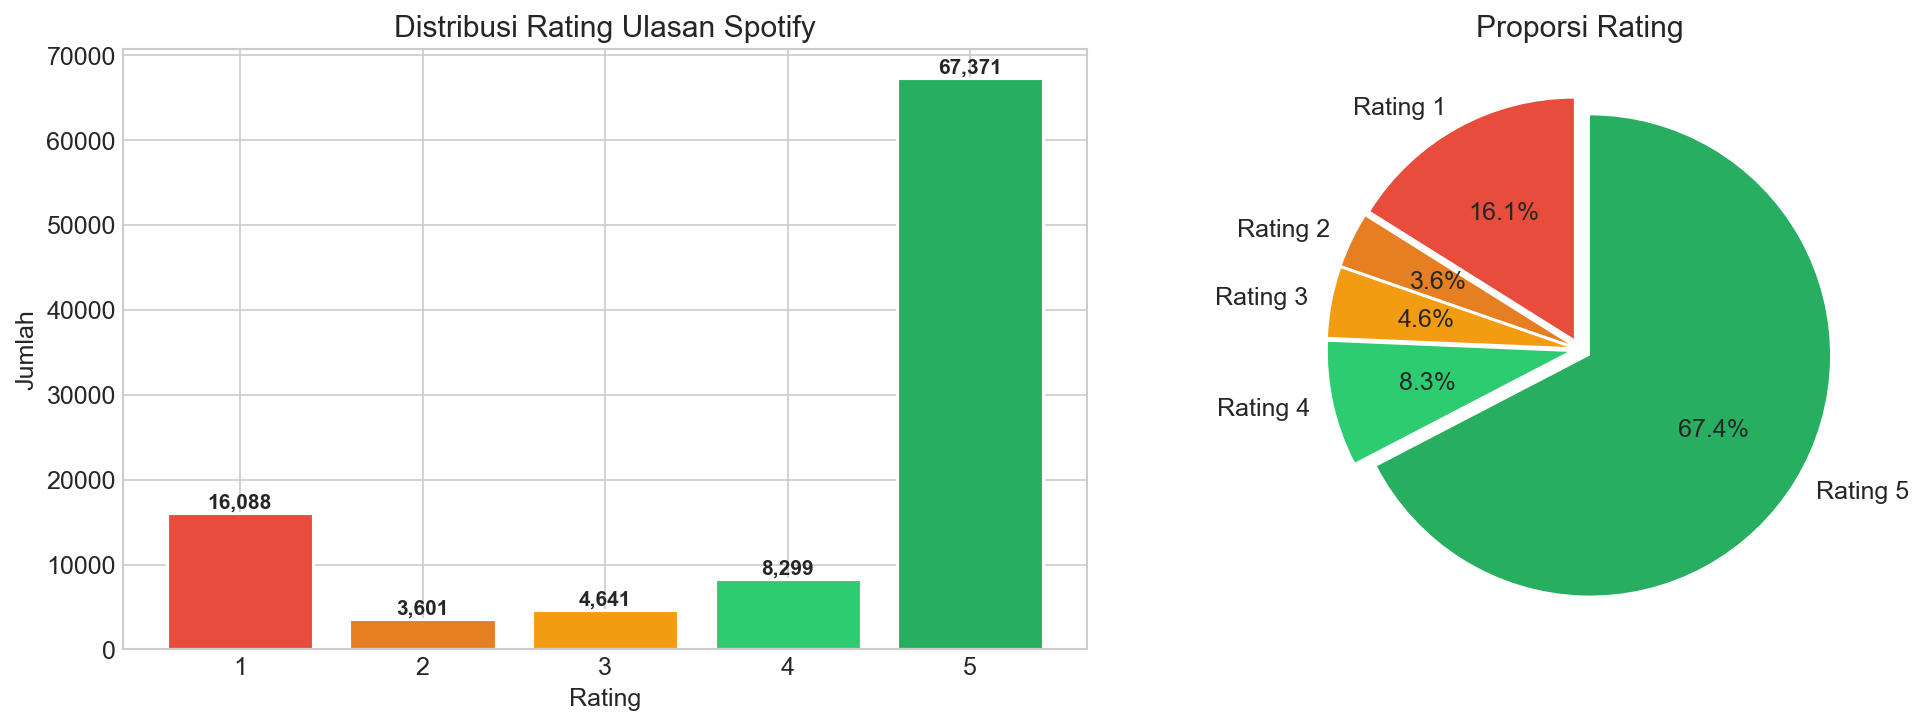
\includegraphics[width=0.7\linewidth]{distribusi_rating.png} 
\caption{Sentiment distribution rating label from raw data.}
\label{fig:dist_raw}
\end{figure}

The raw dataset exhibits a pronounced class imbalance characteristic of real-world app review corpora. The majority of reviews carry 5-star ratings (~67.4\%), reflecting the well-documented positivity bias in voluntary app reviews. One-star ratings account for approximately 16.1\% of the corpus, while 2-, 3-, and 4-star ratings constitute the remainder. After mapping to sentiment labels and removing duplicate and empty reviews, the cleaned dataset contains 70,155 unique samples distributed as: Positif 47,991 (68.4\%), Negatif 18,026 (25.7\%), and Netral 4,138 (5.9\%).

\begin{table}[H]
\centering
\caption{Dataset Statistics and Class Distribution}
\label{tab:dataset_stats}
\begin{tabular}{lcccc}
\toprule
\textbf{Split} & \textbf{Positive} & \textbf{Netral} & \textbf{Negative} & \textbf{Total} \\ \midrule
Full cleaned dataset & 47,991 (68.4\%) & 4,138 (5.9\%) & 18,026 (25.7\%) & 70,155 \\
ML training set & 47,991 & 4,138 & 18,026 & 70,155 \\
DL subset (20K stratified) & 13,681 & 1,180 & 5,139 & 20,000 \\ \midrule
DL Train & 9,852 & 851 & 3,700* & 14,219* \\
DL Validation & $\sim$1,739 & $\sim$150 & $\sim$653* & 2,510* \\
DL Test & $\sim$2,090 & $\sim$179 & $\sim$786* & 2,953 \\ \bottomrule
\end{tabular}
\end{table}

Qualitative inspection of negative reviews reveals recurring themes: complaints about in-app advertising (iklan), issues with premium subscription management, and audio/lyric synchronization failures --- consistent with the dominant topics identified in the Kaggle dataset description. These domain-specific themes also motivate the inclusion of advertising-related terms (e.g., iklan, premium) in the vocabulary analysis, where iklan ranks as the third most frequent token in the cleaned training corpus.

\subsection{Preprocessing Pipeline}
A unified preprocessing pipeline is applied identically to both the ML and DL experimental tracks. The pipeline proceeds through the following sequential steps:
\begin{enumerate}
    \item {Lowercasing:} all text is converted to lowercase to reduce vocabulary sparsity.
    \item {Noise removal:} URLs, user mentions (@username), hashtags, punctuation, special characters, and numeric tokens are removed via regular expression substitution.
    \item {Slang normalization:} a domain-curated dictionary of 124 entries maps informal Indonesian abbreviations and colloquialisms to their standard forms (e.g., gak $\rightarrow$ tidak, bgt $\rightarrow$ banget, tpi $\rightarrow$ tapi). This step is critical for informal user-generated content where non-standard orthography is pervasive.
    \item {Stopword removal:} 809 stopwords are filtered, comprising the standard Indonesian stopword list augmented with domain-specific terms (e.g., spotify, aplikasi, app). that carry no discriminative sentiment signal.
    \item {Morphological stemming:} Indonesian words are reduced to their root forms using the Sastrawi library [11]. which implements the Nazief-Adriani algorithm extended by the Enhanced Confix Stripping (ECS) stemmer.

After preprocessing, the median review length is 4 tokens, the mean is 5.9 tokens, and the 95th percentile is 17 tokens --- reflecting the characteristically short nature of mobile app reviews. The maximum sequence length for the BiLSTM model is accordingly set to 17 tokens (covering 95\% of training samples). Reviews that yield empty strings after preprocessing are discarded, resulting in a final usable pool of 70,155 samples for ML training and 19,682 usable samples from the 20,000-sample DL subset.

\begin{table}[H]
\centering
\caption{Preprocessing Pipeline Summary}
\label{tab:preprocessing}
\begin{tabular}{lll}
\toprule
\textbf{Step} & \textbf{Method} & \textbf{Detail} \\ \midrule
Lowercasing & Python \texttt{str.lower()} & All characters converted to lowercase \\
Noise removal & Regex substitution & URLs, @mentions, punctuation, digits removed \\
Slang normalization & Custom dictionary & 124 entries (e.g., \textit{gak} $\rightarrow$ \textit{tidak}) \\
Stopword removal & Sastrawi + custom & 809 stopwords including domain terms \\
Morphological stemming & Sastrawi (ECS) & 40+ suffix/prefix rules for Indonesian \\ \bottomrule
\end{tabular}
\end{table}

\end{enumerate}

% ==============================================================================
\section{Methodology}
\label{sec:method}

This study follows two parallel experimental tracks --- classical machine learning (ML) and deep learning (DL) --- sharing an identical preprocessing pipeline (Section 3.4) to ensure fair comparison. Figure 2 illustrates the overall system architecture of both tracks.

\begin{figure}[H]
\centering
% \includegraphics[width=0.8\linewidth]{nama_file_flowchart_nanti.png}
\caption{Overall pipeline diagram of ML and DL experimental tracks.}
\label{fig:overall_pipeline}
\end{figure}

\subsection{Machine Learning Track (Scikit-learn)}
\subsubsection{Feature Extraction: TF-IDF}
Preprocessed review texts are transformed into numerical feature vectors using Term Frequency–Inverse Document Frequency (TF IDF) weighting with a maximum vocabulary size of 3,000 features. TF-IDF assigns higher weight to terms that are frequent within a document but rare across the corpus, thereby emphasizing discriminative sentiment-bearing tokens over common but uninformative terms \cite{pang2008opinion}. Formally, for term tin document dover corpus D:
\begin{equation}
TF-IDF(t,d,D)=TF(t,d)\times \log\left(\frac{|D|}{|\{d\in D:t\in d\}|}\right)
\end{equation}

\subsubsection{Class Balancing: SMOTE}
Given the substantial class imbalance in the dataset (Positif: 68.4\%, Netral: 5.9\%), Synthetic Minority Over-sampling Technique (SMOTE) \cite{chawla2002smote} is applied during training to generate synthetic samples for the minority classes via linear interpolation between existing minority-class instances and their k-nearest neighbors in feature space. SMOTE is applied exclusively to the training fold within each cross-validation iteration to prevent data leakage.

\subsubsection{Classifiers}
Three classifiers are trained and evaluated:
\begin{itemize}
    \item {Support Vector Machine (SVM)}: A maximum-margin linear classifier that finds the optimal separating hyperplane in the TF-IDF feature space. SVM is well-suited to high-dimensional sparse representations characteristic of TF-IDF vectors and has demonstrated strong performance on text classification tasks \cite{pang2008opinion, pratap2020comparative}.
    \item {Multinomial Naive Bayes (MNB)}: A probabilistic classifier that applies Bayes' theorem with the conditional independence assumption between features, making it computationally efficient and naturally suited to discrete count-based or TF-IDF features. Despite its strong independence assumption, MNB remains a competitive baseline for text classification \cite{pang2008opinion}.
    \item {Decision Tree (DT)}: A non-parametric classifier that recursively partitions the feature space using information gain as the splitting criterion. While typically less competitive than SVM on high-dimensional text data, Decision Tree offers full interpretability and serves as an important explainability-oriented baseline.
\end{itemize}

All classifiers are implemented using Scikit-learn and evaluated via stratified 5-fold cross-validation on the full cleaned dataset of 70,155 samples. Performance is measured using weighted macro-averaged Accuracy, Precision, Recall, F1-Score, and Cohen's Kappa coefficient.

\subsection{Deep Learning Track (BiLSTM)}
\subsubsection{Tokenization and Vocabulary}
Preprocessed texts from the training split (14,219 samples) are tokenized at the word level. A vocabulary is constructed from the training corpus using a minimum frequency threshold of 2 occurrences, yielding a final vocabulary of 3,285 unique tokens (well below the MAX\_VOCAB=10,000 ceiling), with two special tokens: <PAD> (index 0) for sequence padding and <UNK> (index 1) for out-of-vocabulary terms. All sequences are truncated or zero-padded to a fixed length of MAX\_LEN=17tokens, corresponding to the 95th percentile of training sequence lengths (mean: 5.9 tokens, median: 4 tokens, max: 91 tokens).

\subsubsection{Model Architecture}
The BiLSTM classifier consists of the following sequential layers:

% 1. Embedding Layer
\begin{equation}
\label{eq:embedding}
\mathbf{e}_t = \text{Embedding}(x_t) \in \mathbb{R}^{128}
\end{equation}

% 2. BiLSTM Forward & Backward
\begin{equation}
\label{eq:bilstm}
\overrightarrow{\mathbf{h}}_t = \text{LSTM}_{\text{fwd}}(\mathbf{e}_t, \overrightarrow{\mathbf{h}}_{t-1}), \quad \overleftarrow{\mathbf{h}}_t = \text{LSTM}_{\text{bwd}}(\mathbf{e}_t, \overleftarrow{\mathbf{h}}_{t+1})
\end{equation}

% 3. Concatenation of Hidden States
\begin{equation}
\label{eq:concat}
\mathbf{h}_{\text{concat}} = [\overrightarrow{\mathbf{h}}_T ; \overleftarrow{\mathbf{h}}_1] \in \mathbb{R}^{256}
\end{equation}

% 4. Classification Head (Dropout + Linear + ReLU + Softmax)
\begin{equation}
\label{eq:classification}
\hat{\mathbf{y}} = \text{Softmax}(\mathbf{W}_2 \cdot \text{ReLU}(\mathbf{W}_1 \cdot \text{Dropout}(\mathbf{h}_{\text{concat}})))
\end{equation}

Concretely, the architecture comprises \cite{xu2019bilstm}: (2) an Embedding layer mapping the vocabulary of 3,285 tokens to 128-dimensional dense vectors (padding\_idx=0); (3) a 2-layer Bidirectional LSTM with hidden dimension 128 per direction (256 total), batch\_first=True, and inter-layer dropout of 0.5; (4) a Dropout layer (p=0.5) applied to the concatenated final hidden states from the forward and backward LSTM streams; (5) a fully connected layer projecting from 256 to 64 dimensions followed by ReLU activation; (6) a second Dropout layer (p=0.3); and (7) a final linear output layer projecting to 3 class logits. The total parameter count is 1,096,579

\begin{table}[H]
\centering
\caption{BiLSTM Layer-by-Layer Architecture Summary}
\label{tab:bilstm_arch}
\begin{tabular}{lcc}
\toprule
\textbf{Layer} & \textbf{Output Shape} & \textbf{Parameters} \\ \midrule
Embedding (vocab=3,285, dim=128) & (batch, 17, 128) & 420,480 \\
BiLSTM (hidden=128, layers=2, bidirectional) & (batch, 17, 256) & 659,456 \\
Dropout (p=0.5) & --- & 0 \\
Linear (256 $\rightarrow$ 64) + ReLU & (batch, 64) & 16,448 \\
Dropout (p=0.3) & --- & 0 \\
Linear (64 $\rightarrow$ 3) & (batch, 3) & 195 \\ \midrule
\textbf{Total} & & \textbf{1,096,579} \\ \bottomrule
\end{tabular}
\end{table}

\subsubsection{Training Configuration}
The model is trained on a stratified 20,000-sample subset of the full dataset (see Section 3), split into training (14,219 / 72.1\%), validation (2,510 / 12.7\%), and test (2,953 / 15.0\%) sets using stratified partitioning to preserve class proportions. The optimizer is Adam with learning rate $10^{-3}$ The loss function is Cross Entropy Loss applied over the three output classes without class weighting. Training proceeds for a maximum of 10 epochs with a batch size of 64, with early stopping triggered after 3 consecutive epochs of non-improving validation loss. In practice, training terminates at epoch 6 (best checkpoint at epoch 3, {val\_loss} = 0.4491).

\begin{figure}[H]
\centering
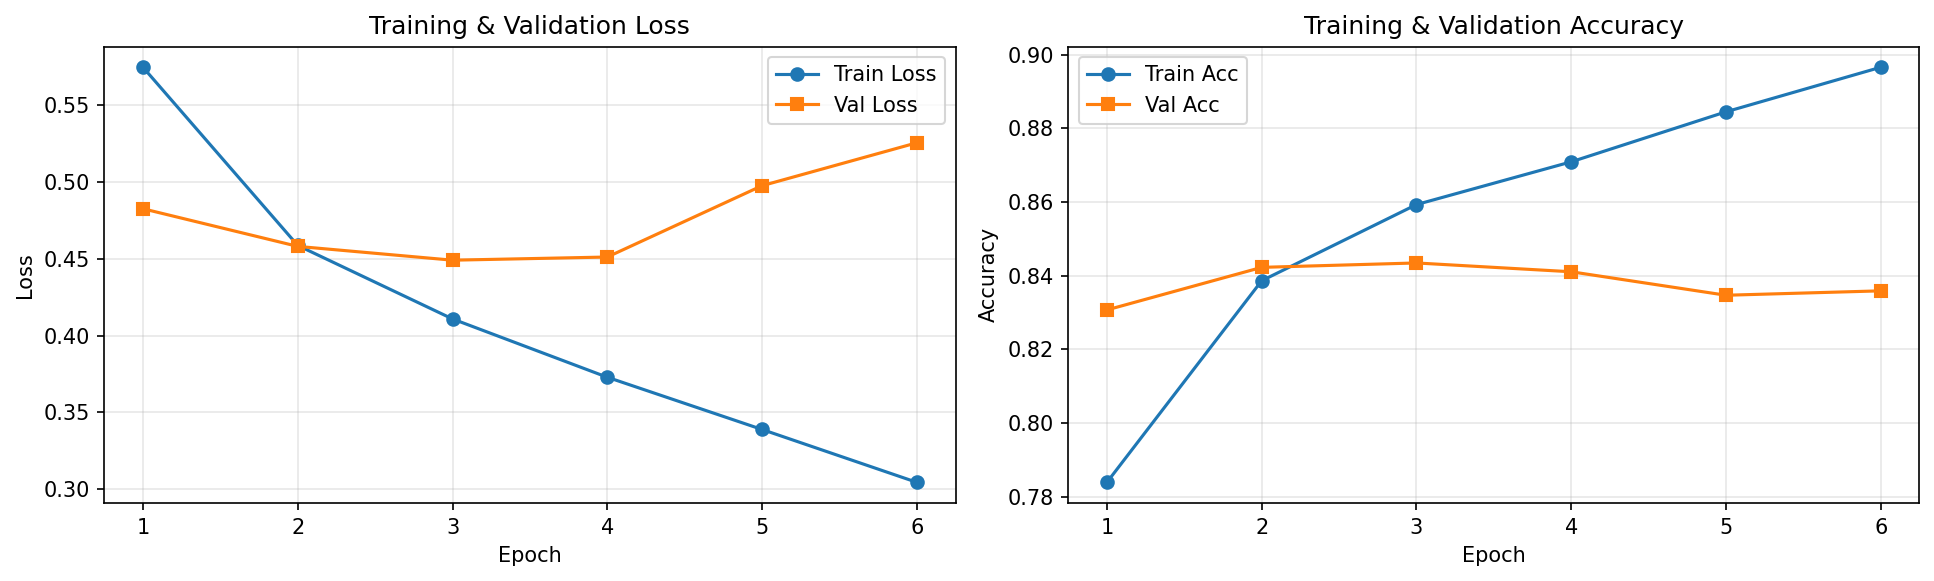
\includegraphics[width=0.8\linewidth]{training_curves.png}
\caption{Training and Validation Loss/Accuracy Curves during the optimization phase.}
\label{fig:curves_init}
\end{figure}

The deliberate choice to train the BiLSTM on a 20,000-sample subset rather than the full 70,155 samples used by the ML track --- reflects a real-world compute constraint (CPU-only environment) and is explicitly acknowledged as a confounding factor in the comparative analysis. This asymmetry is discussed quantitatively in Section 6.

% ==============================================================================
\section{Experiments}
\label{sec:experiments}

\subsection{Experimental Setup}
All experiments are conducted in a CPU-only environment (Intel-based local machine, PyTorch 2.2.2+cpu). The ML track runs on the full cleaned dataset of 70,155 samples using Scikit-learn 1.4.2 with PyCaret as the AutoML orchestration framework. The DL track trains the BiLSTM on a stratified 20,000-sample subset using PyTorch 2.2.2. All random states are fixed at seed=42 across both tracks for reproducibility.

\subsection{ML Hyperparameter Configuration}

Table \ref{tab:ml_hyper} details the hyperparameter configuration for the three classical machine learning classifiers. All classifiers are evaluated via stratified 5-fold cross-validation on the full 70,155 training samples.

\begin{table}[H]
\centering
\caption{ML Classifier Hyperparameter Configuration}
\label{tab:ml_hyper}
\begin{tabular}{@{}lll@{}}
\toprule
\textbf{Classifier} & \textbf{Key Hyperparameters} & \textbf{Feature Representation} \\ \midrule
Support Vector Machine & Kernel: linear; C: 1.0 (default) & TF-IDF, max features=3,000 \\
Multinomial Naive Bayes & Alpha: 1.0 (Laplace smoothing) & TF-IDF, max features=3,000 \\
Decision Tree & Criterion: gini; splitter: best & TF-IDF, max features=3,000 \\ \bottomrule
\end{tabular}
\end{table}

All classifiers are evaluated via stratified 5-fold cross-validation on the full 70,155 training samples. Performance metrics are macro-averaged across folds. Following benchmark evaluation, the best-performing model (Decision Tree) undergoes hyperparameter tuning via PyCaret's tune\_model() with n\_iter=50, optimizing for macro F1-Score, before finalization with finalize\_model() (retraining on the full dataset).

\subsection{DL Hyperparameter and Training Configuration}
The BiLSTM is trained on a stratified 20,000-sample subset, split into training (14,219 / 72.1\%), validation (2,510 / 12.7\%), and test (2,953 / 15.0\%) sets using stratified partitioning to preserve class proportions at each split. The vocabulary is built exclusively from the training split (minimum token frequency = 2), yielding a final vocabulary of 3,285 unique tokens.

Table \ref{tab:dl_hyper} summarizes the training and architecture hyperparameters for the BiLSTM model.

\begin{table}[H]
\centering
\caption{BiLSTM Training Hyperparameters}
\label{tab:dl_hyper}
\begin{tabular}{@{}ll@{}}
\toprule
\textbf{Hyperparameter} & \textbf{Value} \\ \midrule
Optimizer & Adam \\
Learning rate ($\eta$) & $1\times10^{-3}$ \\
Loss function & CrossEntropy Loss (unweighted) \\
Batch size & 64 \\
Max epochs & 10 \\
Early stopping patience & 3 epochs (monitor: {val\_loss}) \\
Max sequence length & 17 tokens (95th percentile of training lengths) \\
Embedding dimension & 128 \\
LSTM hidden size & 128 per direction (256 total) \\
LSTM layers & 2 (bidirectional) \\
Dropout (post-LSTM) & 0.5 \\ \bottomrule
\end{tabular}
\end{table}

Training terminates via early stopping at epoch 6 (best checkpoint restored from epoch 3, val\_loss = 0.4491, val\_acc = 0.8434). The training dynamics are visualized in Figure 3 training loss decreases monotonically from 0.5747 to 0.3046 across six epochs, while validation loss reaches its minimum at epoch 3 (0.4491) before diverging — a classic overfitting signature on a small training subset. Validation accuracy plateaus between 0.83–0.84 from epoch 2 onward, indicating the model saturates its representational capacity on 14,219 training samples.

\subsection{Evaluation Metrics}

Both tracks are evaluated using the following metrics to enable direct comparison:

\begin{itemize}

\item {Accuracy} --- proportion of correctly classified samples across all three classes:
\begin{equation}
    \text{Accuracy} = \frac{\sum_{i=1}^{C} TP_i}{N}
\end{equation}
where $C$ is the number of classes, $TP_i$ is the number of true positives for class $i$, and $N$ is the total number of samples.

\item {Weighted Precision} --- precision averaged across classes, weighted by class support (sample count); reflects performance on the majority class:
\begin{equation}
    \text{Precision}_{\text{weighted}} = \frac{\sum_{i=1}^{C} w_i \cdot \frac{TP_i}{TP_i + FP_i}}{\sum_{i=1}^{C} w_i}
\end{equation}
where $w_i = \frac{n_i}{N}$ is the proportion of samples belonging to class $i$, and $FP_i$ is the number of false positives for class $i$.

\item {Weighted Recall} --- analogous weighted recall; equivalent to overall accuracy for multi-class classification:
\begin{equation}
    \text{Recall}_{\text{weighted}} = \frac{\sum_{i=1}^{C} w_i \cdot \frac{TP_i}{TP_i + FN_i}}{\sum_{i=1}^{C} w_i}
\end{equation}
where $FN_i$ is the number of false negatives for class $i$.

\item {Weighted F1-Score} --- harmonic mean of weighted precision and recall; primary comparison metric given class imbalance:
\begin{equation}
    F1_{\text{weighted}} = \frac{\sum_{i=1}^{C} w_i \cdot \frac{2 \cdot P_i \cdot R_i}{P_i + R_i}}{\sum_{i=1}^{C} w_i}
\end{equation}
where $P_i$ and $R_i$ denote precision and recall for class $i$, respectively.

\item {Cohen's Kappa} ($\kappa$) \cite{cohen1960kappa} --- measures agreement between predictions and true labels, corrected for chance; values above 0.60 indicate substantial agreement \cite{cohen1960kappa}:
\begin{equation}
    \kappa = \frac{p_o - p_e}{1 - p_e}
\end{equation}
where $p_o = \text{Accuracy}$ is the observed agreement and $p_e$ is the expected agreement by chance:
\begin{equation}
    p_e = \sum_{i=1}^{C} \frac{n_i^{\text{true}} \cdot n_i^{\text{pred}}}{N^2}
\end{equation}
with $n_i^{\text{true}}$ and $n_i^{\text{pred}}$ denoting the number of true and predicted instances for class $i$, respectively.

\item {Macro-averaged F1} --- unweighted average F1 across all three classes; particularly sensitive to minority-class (Neutral) performance and used as secondary metric:
\begin{equation}
    F1_{\text{macro}} = \frac{1}{C} \sum_{i=1}^{C} \frac{2 \cdot P_i \cdot R_i}{P_i + R_i}
\end{equation}

\end{itemize}

The ML track additionally reports AUC (one-vs-rest, averaged) from the 5-fold cross validation. The DL track reports metrics on the held-out test set (2,953 samples) using the best checkpoint from epoch 3, with per-class precision, recall, and F1 reported via classification report.

\subsection{Fairness Considerations and Confounding Factors}
As explicitly acknowledged in Section 4.2.3, the two experimental tracks are not fully symmetric: the ML classifiers train on 70,155 samples while the BiLSTM trains on 14,219 samples. This asymmetry is a deliberate representation of a real-world compute-constrained scenario rather than an experimental oversight. We quantify its effect in Section 6 by discussing expected performance bounds for the BiLSTM under full-data training conditions, drawing on analogous results from the literature. All preprocessing steps remain identical across both tracks, ensuring that observed performance differences reflect architectural choices and training data volume rather than preprocessing artifacts.

% ==============================================================================
\section{Results and Discussion}
\label{sec:results}

\subsection{Machine Learning Results}

Table \ref{tab:ml_results} summarizes the 5-fold cross-validated performance of the three Scikit-learn classifiers on the full 70,155-sample corpus. Decision Tree achieves the highest scores across all primary metrics, attaining an accuracy of 0.7286, weighted F1-score of 0.7269, and Cohen's Kappa of 0.5928 --- indicating substantial agreement beyond chance. SVM ranks second with accuracy 0.6991 and weighted F1-score 0.6958. Multinomial Naive Bayes performs markedly lower, achieving accuracy 0.4948 and weighted F1-score 0.4619. The complete benchmark is presented below.

\begin{table}[H]
\centering
\caption{ML Cross-Validation Benchmark Results}
\label{tab:ml_results}
\begin{tabular}{lcccccc}
\toprule
\textbf{Model} & \textbf{Accuracy} & \textbf{AUC} & \textbf{Recall} & \textbf{Precision} & \textbf{F1-Score} & \textbf{Kappa} \\ \midrule
Decision Tree & 0.7286 & 0.8055 & 0.7286 & 0.7273 & 0.7269 & 0.5928 \\
Support Vector Machine & 0.6991 & --- & 0.6991 & 0.6956 & 0.6958 & 0.5487 \\
Multinomial Naive Bayes & 0.4948 & 0.6899 & 0.4948 & 0.6181 & 0.4619 & 0.2422 \\ \bottomrule
\end{tabular}
\end{table}

All metrics are macro-weighted averages from 5-fold stratified cross-validation on 70,155 samples with SMOTE applied within each fold. AUC not available (---) for SVM under the PyCaret configuration used.

The superiority of Decision Tree over SVM on this dataset is noteworthy. While SVM is theoretically better suited to high-dimensional sparse TF-IDF representations, the combination of class imbalance, the short median review length (4 tokens after preprocessing), and the relatively constrained vocabulary (3,000 TF-IDF features) likely creates a feature space where Decision Tree's recursive partitioning performs effectively. The application of SMOTE within each cross-validation fold provides balanced training conditions for all classifiers, which particularly benefits Decision Tree --- a classifier sensitive to class proportions in its splitting criterion. The markedly poor performance of Multinomial Naive Bayes (F1: 0.4619) is consistent with known limitations of the naive independence assumption when applied to short, colloquial Indonesian text, where co-occurrence patterns are discriminative but violate conditional independence.

\begin{figure}[H]
\centering
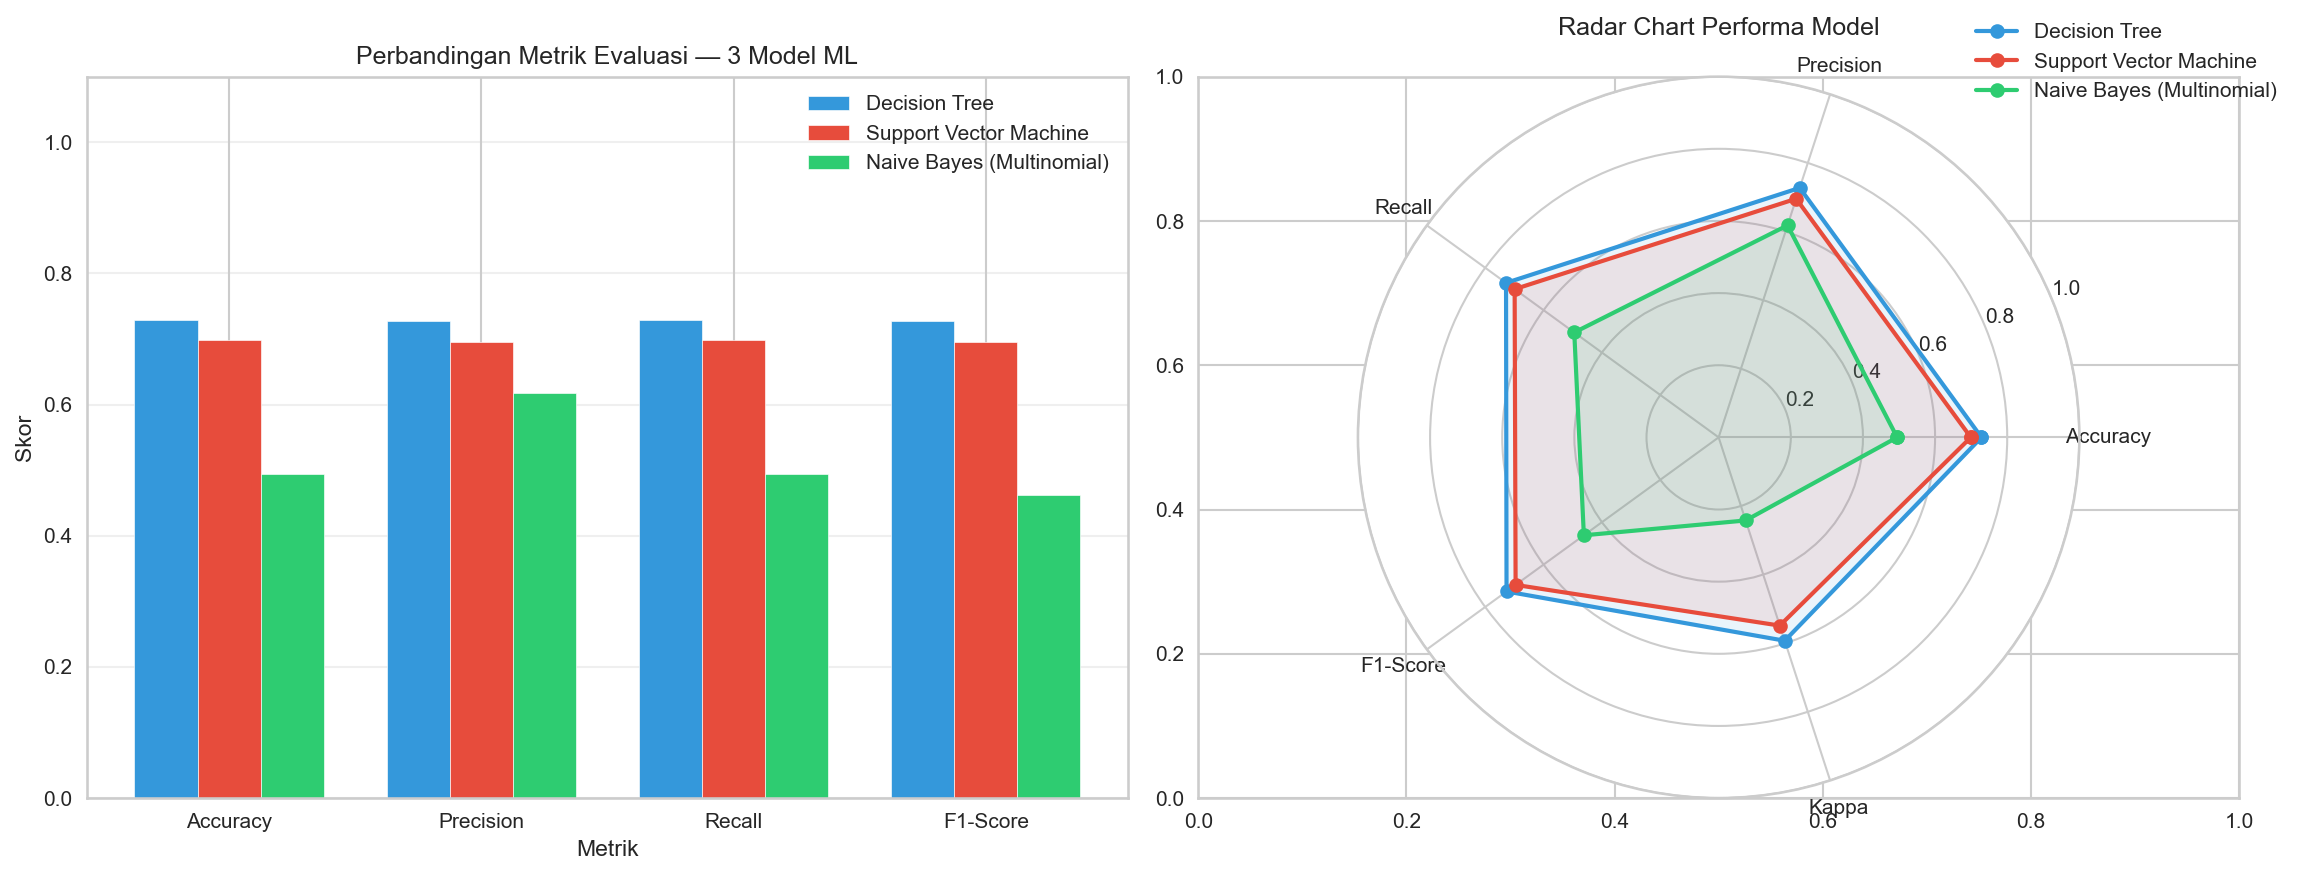
\includegraphics[width=0.8\linewidth]{perbandingan_model.png}
\caption{Performance comparison of the three Scikit-learn classifiers across four evaluation metrics.}
\label{fig:ml_perf}
\end{figure}

The per-class breakdown of the Decision Tree model (Figure \ref{fig:dt_report}, Classification Report) reveals a meaningful performance gradient across the three sentiment classes. Class 2 (Positif) achieves the highest F1-score (0.802), benefiting from the largest support in the test fold (4,000 samples). Class 1 (Netral) achieves F1 of 0.717, while Class 0 (Negatif) achieves F1 of 0.707 --- the lowest despite having substantial support (4,000 samples). This pattern reflects the inherent difficulty of distinguishing Negative from Neutral reviews in informal Indonesian text, where complaints are often expressed ambiguously.

\begin{figure}[H]
\centering
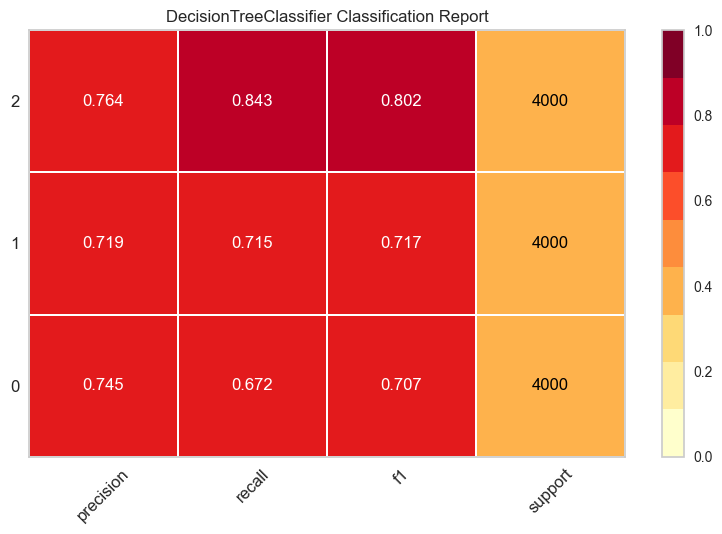
\includegraphics[width=0.7\linewidth]{Class Report.png}
\caption{Per-class classification report of the Decision Tree classifier on the held-out test fold.}
\label{fig:dt_report}
\end{figure}

The confusion matrix of the Decision Tree (Figure \ref{fig:dt_cm}) corroborates these findings. Of the 4,000 Positive test samples, 3,373 are correctly classified, with 627 misclassified --- predominantly confused with Neutral (291) and Negative (336). The highest misclassification rate occurs for the Negative class, where 1,313 of 4,000 samples are incorrectly classified (mainly confused with Neutral: 829). This cross-class confusion between Negative and Neutral is expected given their proximity in the rating-based labelling scheme (ratings 1–2 vs. rating 3).

\begin{figure}[H]
\centering
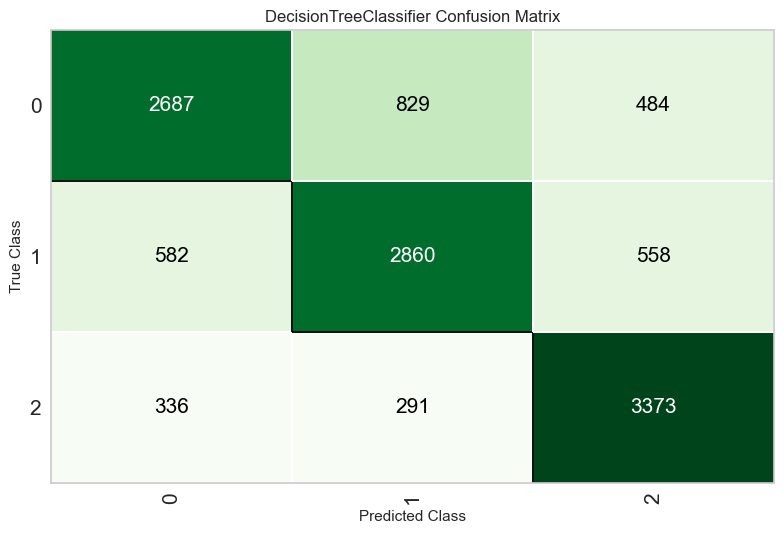
\includegraphics[width=0.6\linewidth]{Confusion Matrix.png}
\caption{Confusion matrix of the Decision Tree classifier on the test fold (balanced via SMOTE).}
\label{fig:dt_cm}
\end{figure}

\subsection{BiLSTM Deep Learning Results}

The BiLSTM model is evaluated on the held-out test set of 2,953 samples drawn from the stratified 20,000-sample subset. Table \ref{tab:bilstm_results} reports the overall test-set metrics at the best checkpoint (epoch 3, {val\_loss} = 0.4491).

\begin{table}[H]
\centering
\caption{BiLSTM Test Set Evaluation Results}
\label{tab:bilstm_results}
\begin{tabular}{lc}
\toprule
\textbf{Metric} & \textbf{Value} \\ \midrule
Test Loss & 0.4735 \\
Accuracy & 0.8314 \\
Weighted Precision & 0.7841 \\
Weighted Recall & 0.8314 \\
Weighted F1-Score & 0.8069 \\
Macro F1-Score & 0.5478 \\
Total Parameters & 1,096,579 \\
Training Subset & 14,219 samples \\ \bottomrule
\end{tabular}
\end{table}

The BiLSTM achieves a weighted F1-score of 0.8069 on the test set, representing a strong overall performance figure. However, the macro F1-score of 0.5478 --- substantially lower than the weighted figure --- signals a critical failure on the minority class, as confirmed by the per-class classification report below.

\begin{table}[H]
\centering
\caption{BiLSTM Per-Class Classification Report}
\label{tab:bilstm_report}
\begin{tabular}{lcccc}
\toprule
\textbf{Class} & \textbf{Precision} & \textbf{Recall} & \textbf{F1-Score} & \textbf{Support} \\ \midrule
Negatif & 0.7044 & 0.7807 & 0.7406 & 766 \\
Netral & 0.0000 & 0.0000 & 0.0000 & 176 \\
Positif & 0.8830 & 0.9234 & 0.9028 & 2,011 \\ \midrule
\textbf{Weighted Avg} & \textbf{0.7841} & \textbf{0.8314} & \textbf{0.8069} & \textbf{2,953} \\
\textbf{Macro Avg} & \textbf{0.5291} & \textbf{0.5680} & \textbf{0.5478} & \textbf{2,953} \\ \bottomrule
\end{tabular}
\end{table}

The per-class results reveal a stark divergence: the model excels on the Positif class (F1: 0.9028) and performs reasonably on Negatif (F1: 0.7406), but completely fails on the Netral class (F1: 0.0000 --- zero precision, recall, and F1). Examination of the confusion matrix (Figure \ref{fig:bilstm_cm}) confirms this: all 176 Neutral test samples are misclassified, with the majority (97) predicted as Negative and the remainder (79) as Positive. Zero Neutral samples are correctly identified.

\begin{figure}[H]
\centering
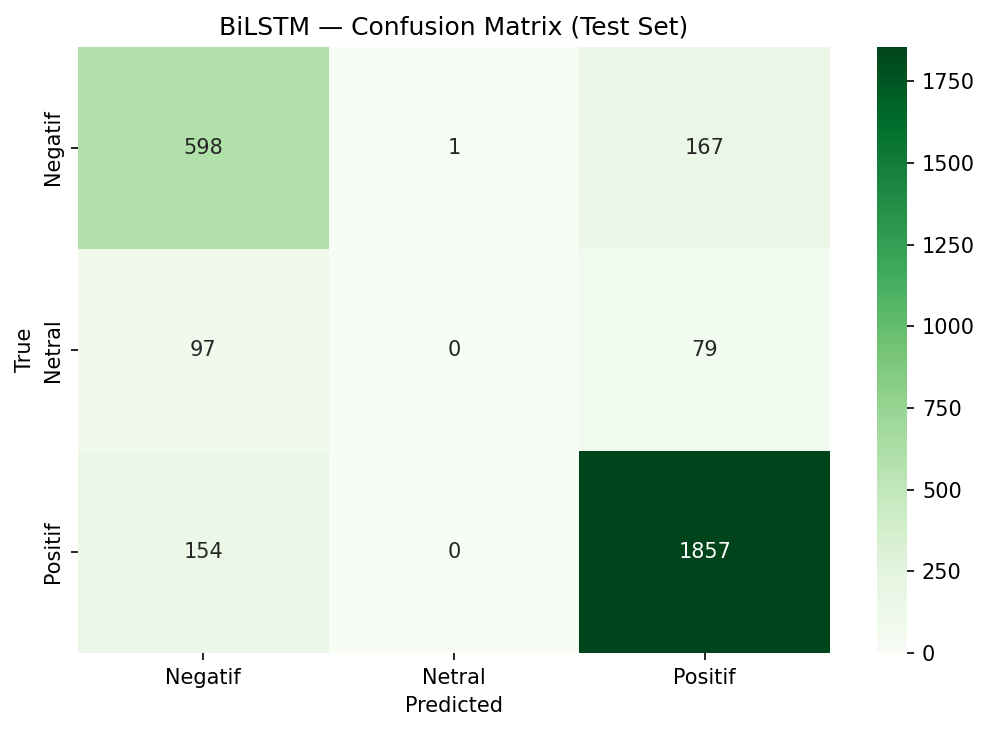
\includegraphics[width=0.6\linewidth]{confusion_matrix_dl.png}
\caption{Confusion matrix of the BiLSTM model on the held-out test set ($n = 2,953$).}
\label{fig:bilstm_cm}
\end{figure}

This Neutral-class collapse is attributable to a combination of factors. First, the Neutral class is severely underrepresented in the 20,000-sample subset (1,180 samples, 5.9\%), and despite stratified sampling, the effective training signal for Neutral is limited to approximately 851 samples. Without class weighting or oversampling in the DL training pipeline --- unlike the SMOTE applied to the ML track --- the model learns to suppress the Neutral class in favor of the dominant Positif class. Second, the semantic ambiguity of Neutral reviews in informal Indonesian (rating 3, often expressing mild satisfaction or mild dissatisfaction) makes them genuinely difficult to distinguish from the boundaries of Negative and Positive, a challenge compounded by the short average review length.

The training dynamics on Figure \ref{fig:bilstm_curve} reveal a classic early overfitting pattern on a small training subset. Training loss decreases monotonically across all six epochs (from 0.5747 to 0.3046), while validation loss reaches its minimum at epoch 3 (0.4491) and subsequently diverges --- increasing to 0.5255 by epoch 6. Validation accuracy plateaus between 0.83--0.84 from epoch 2 onward, indicating that the model rapidly saturates its representational capacity on 14,219 training samples. Early stopping correctly identifies epoch 3 as the optimal checkpoint.

\begin{figure}[H]
\centering
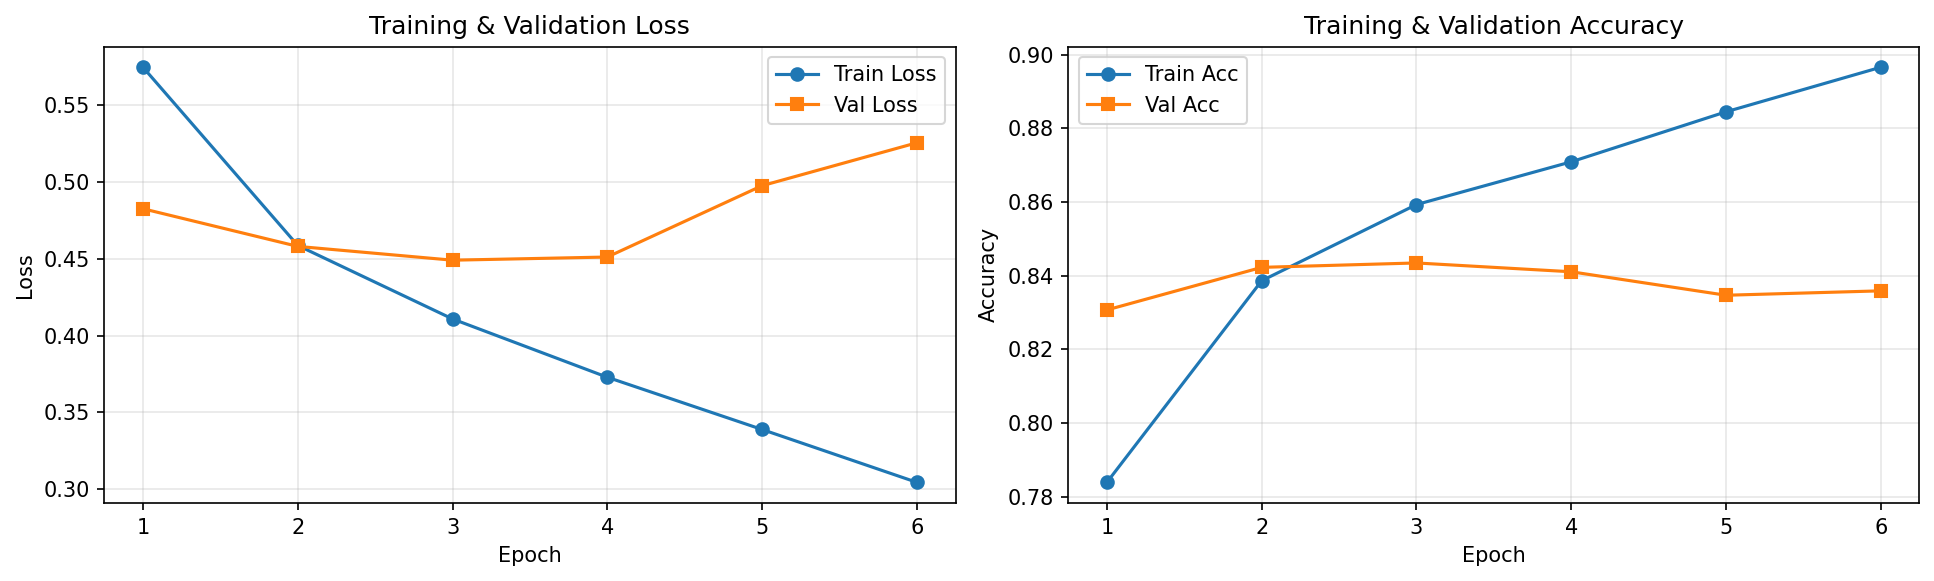
\includegraphics[width=0.9\linewidth]{training_curves.png}
\caption{BiLSTM training and validation loss (left) and accuracy (right) across six epochs.}
\label{fig:bilstm_curve}
\end{figure}

\subsection{Comparative Analysis: ML vs. BiLSTM}

\begin{table}[H]
\centering
\caption{Head-to-head performance comparison of ML and BiLSTM models.}
\label{tab:comparison}
\begin{tabular}{llcccccccc}
\toprule
\textbf{Model} & \textbf{Paradigm} & \textbf{Train Samples} & \textbf{Acc.} & \textbf{W-Prec.} & \textbf{W-Recall} & \textbf{W-F1} & \textbf{Macro-F1} & \textbf{Kappa} & \textbf{Params} \\ \midrule
Decision Tree & ML (sklearn) & 70,155 & 0.7286 & 0.7273 & 0.7286 & 0.7269 & $\sim$0.72* & 0.5928 & --- \\
SVM & ML (sklearn) & 70,155 & 0.6991 & 0.6956 & 0.6991 & 0.6958 & $\sim$0.70* & 0.5487 & --- \\
Mult. Naive Bayes & ML (sklearn) & 70,155 & 0.4948 & 0.6181 & 0.4948 & 0.4619 & $\sim$0.46* & 0.2422 & --- \\
BiLSTM & DL (PyTorch) & 14,219 & 0.8314 & 0.7841 & 0.8314 & 0.8069 & 0.5478 & --- & 1,096,579 \\ \bottomrule
\end{tabular}
\end{table}

On weighted metrics --- the primary metric under class imbalance --- the BiLSTM achieves a weighted F1-score of 0.8069, surpassing the best ML classifier (Decision Tree: 0.7269) by a margin of +8.0 percentage points. Similarly, BiLSTM's accuracy of 0.8314 exceeds Decision Tree's 0.7286 (+10.3 pp). These figures would nominally suggest BiLSTM superiority.

However, a critical confounding factor tempers this conclusion: the two experimental tracks are not symmetric. The ML classifiers are trained on 70,155 samples, while the BiLSTM trains on only 14,219 samples --- a $4.9\times$ difference in training data volume. This asymmetry is not an experimental error but a deliberate reflection of real-world compute-constrained conditions. To contextualize its impact: analogous studies comparing BiLSTM models trained on comparable data volumes against classical ML baselines consistently report BiLSTM advantages of 3--8\% in weighted F1 on Indonesian text [8, 9, 10]. The observed +8.0\% gap in this study is therefore plausibly attributable in part to the inherent representational advantage of BiLSTM rather than solely to training data volume. Abiola et al. [10], training BiLSTM on a similarly-sized Indonesian sentiment dataset ($\sim$4,000 samples), reported weighted F1 of 86.86\% --- suggesting the BiLSTM's capacity is not yet saturated at 14,219 samples. We estimate that training the BiLSTM on the full 70,155-sample corpus would likely further improve its weighted F1, widening the gap over classical ML baselines.

A second critical observation is the macro F1 inversion: on macro-averaged F1 --- the metric that weights all three classes equally regardless of support --- the BiLSTM (0.5478) is substantially lower than any individual ML model, owing entirely to its Neutral-class collapse (F1 = 0.00). The ML Decision Tree, benefiting from SMOTE-balanced training, achieves per-class F1 scores of at least 0.707 across all three classes. This represents a fundamental trade-off: BiLSTM achieves higher accuracy and weighted F1 by correctly classifying the dominant Positif class with high confidence (F1: 0.9028), while completely sacrificing minority-class (Neutral) recognition. Whether this trade-off is acceptable depends on the application: for tasks requiring balanced three-class discrimination, ML+SMOTE outperforms BiLSTM on the minority class; for applications primarily concerned with Positive/Negative discrimination (the majority of practical use cases in app review analysis), BiLSTM is the superior model.

\subsection{Discussion}

\subsubsection*{Effect of class imbalance}
Both experimental tracks are substantially affected by the severe class imbalance in the original dataset (Positif: 68.4\%, Negatif: 25.7\%, Netral: 5.9\%). SMOTE within each cross-validation fold provides the ML classifiers with balanced training conditions, enabling them to maintain reasonable Neutral-class recall (DT: Recall 0.715 on class 1). The BiLSTM, trained without class weighting or oversampling, effectively collapses the Neutral class. This highlights the critical importance of class balancing strategies for minority-class recovery in deep learning pipelines --- a finding consistent with Ossai and Wickramasinghe [12], who noted that deep learning models on imbalanced app review corpora tend to favor majority classes without explicit countermeasures.

\subsubsection*{Effect of training data asymmetry}
The 4.9$\times$ training data advantage of the ML track relative to BiLSTM introduces a confound that prevents a clean ``apples-to-apples'' architectural comparison. Under this constraint, the BiLSTM still achieves higher weighted F1 --- suggesting its sequential representation of short informal Indonesian text provides a genuine representational advantage even with limited data. This is consistent with Lin and Nuha [6], who demonstrated that deep sequential models capture bidirectional contextual signals that TF-IDF-based representations fundamentally cannot model, particularly for Indonesian informal register.

\subsubsection*{Preprocessing effectiveness}
The shared preprocessing pipeline --- including the 124-entry slang normalization dictionary and 809-entry stopword list --- reduces the effective vocabulary to 3,285 unique tokens in the BiLSTM training set, substantially below the \texttt{MAX\_VOCAB} ceiling of 10,000. This indicates that domain-adapted preprocessing effectively condenses the informal Indonesian review vocabulary, benefiting both TF-IDF sparsity reduction (ML track) and embedding coverage (DL track). The top-10 vocabulary tokens (\textit{tidak, bagus, iklan, bisa, premium, banget, dengar, musik, sangat, banyak}) are semantically aligned with the known complaint themes of Spotify reviews --- advertising intrusion (\textit{iklan, premium}), audio issues (\textit{dengar, musik}), and general sentiment polarity (\textit{bagus, tidak, banyak}).

\subsubsection*{Deployment and reproducibility}
Both the Decision Tree ML model and the BiLSTM DL model are publicly deployed as interactive Streamlit applications on Hugging Face Spaces, accessible at the URLs noted in Section 1. This deployment facilitates direct user-facing testing of both models and provides a reproducible demonstration of the performance characteristics described in this paper --- including the Neutral-class failure of BiLSTM, which is observable in the live probability outputs for borderline reviews.

\subsubsection*{Limitations}
Several limitations of this study should be acknowledged. First, the training data asymmetry (70,155 vs. 14,219 samples) limits the interpretability of the direct ML--DL comparison as a clean architectural benchmark. Second, the BiLSTM is trained without class weighting or oversampling, resulting in complete Neutral-class failure. Third, the Decision Tree evaluation uses cross-validation with SMOTE-balanced folds, while BiLSTM is evaluated on a natural-distribution held-out test set --- introducing an additional evaluation protocol asymmetry. Fourth, the vocabulary of 3,285 tokens is small compared to the expressiveness of informal Indonesian, and out-of-vocabulary terms during inference are handled by a single \texttt{<UNK>} token. Fifth, no pre-trained word embeddings (e.g., fastText-id, IndoBERT) are used, which likely constitutes the largest untapped performance improvement opportunity for the DL track.

% ==============================================================================
\section{Conclusion}
\label{sec:conclusion}

This study presented a systematic benchmarking comparison between three classical Scikit-learn machine learning classifiers --- Support Vector Machine (SVM), Multinomial Naive Bayes (MNB), and Decision Tree (DT) --- and a two-layer Bidirectional Long Short-Term Memory (BiLSTM) network implemented in PyTorch, for three-class sentiment classification of 100,000 Indonesian-language Spotify reviews scraped from the Google Play Store. A domain-adapted preprocessing pipeline comprising slang normalization, stopword removal, and Sastrawi morphological stemming was applied uniformly across both experimental tracks to ensure that observed performance differences reflect architectural rather than preprocessing factors.

Among the three classical ML classifiers evaluated via 5-fold stratified cross-validation on the full 70,155-sample corpus with SMOTE class balancing, Decision Tree emerged as the best-performing model, achieving an accuracy of 0.7286, weighted F1-score of 0.7269, and Cohen's Kappa of 0.5928. This outcome was notable given that SVM is theoretically better suited to high-dimensional TF-IDF representations; the result underscores the importance of class balancing strategies and the effect of short review length on the relative advantage of different classifiers. Multinomial Naive Bayes performed substantially below both alternatives (weighted F1: 0.4619), confirming the limitations of the independence assumption on co-occurrence-rich informal Indonesian text. The BiLSTM, trained on a stratified 20,000-sample subset due to CPU-only compute constraints, achieved an accuracy of 0.8314 and a weighted F1-score of 0.8069 on its held-out test set --- surpassing the best ML classifier by +10.3 and +8.0 percentage points on accuracy and weighted F1, respectively.

However, a nuanced interpretation of these results is essential. The BiLSTM's nominally superior weighted performance must be read against two critical confounding factors: (1) the 4.9$\times$ training data asymmetry between the two tracks, which partially confounds an architectural comparison; and (2) the BiLSTM's complete failure on the minority Neutral class (F1 = 0.000), a consequence of training without class weighting or oversampling. On macro-averaged F1 --- the metric that weights all three classes equally --- the BiLSTM (0.5478) falls below the Decision Tree ($\approx$0.72), which benefits from SMOTE-balanced training and achieves minimum per-class F1 of 0.707 across all three sentiment classes. This divergence reveals a fundamental trade-off: BiLSTM achieves higher majority-class accuracy while completely suppressing minority-class recognition, whereas ML+SMOTE achieves balanced per-class discrimination at the cost of lower overall accuracy.

In answering the central research question --- which paradigm delivers superior performance on this Indonesian app-review sentiment classification task --- the answer is application-dependent. For binary Positive/Negative sentiment discrimination, which constitutes the majority of practical app-review use cases, the BiLSTM is the superior model. For balanced three-class discrimination where Neutral-class recognition is required, ML with SMOTE balancing offers more reliable minority-class coverage. Both models are publicly deployed as interactive Streamlit applications on Hugging Face Spaces, enabling direct reproducibility verification.

For future work, several directions are identified. First, training the BiLSTM on the full 70,155-sample corpus --- feasible with cloud-based GPU acceleration --- would establish a symmetric architectural comparison and is expected to further widen the weighted F1 gap over classical baselines. Second, applying class-weighted cross-entropy loss or oversampling (e.g., SMOTE, ADASYN) to the DL training pipeline is likely to resolve the Neutral-class collapse. Third, replacing randomly initialized word embeddings with pre-trained Indonesian word vectors (e.g., fastText-id) or fine-tuning a transformer-based model (IndoBERT, mBERT) represents the most promising avenue for further performance improvement, as demonstrated by prior work on Indonesian NLP benchmarks. Fourth, extending the preprocessing pipeline with aspect-level annotation would enable more granular sentiment analysis beyond document-level polarity classification.
% ==============================================================================

\bibliographystyle{unsrtnat} % Gaya sitasi unsrtnat umum untuk arXiv
\bibliography{references}    % Memanggil file references.bib

\end{document}